% !TEX root = ../intro-stellar-physics.tex

The depletion of hydrogen in the core heralds the end of the star's placid main-sequence life. We shall first give an overview of the changes that ensue. Fusion of helium requires a temperature $\gtrsim\val{10^{8}}{\K}$, substantially higher than that required for the fusion of hydrogen. As a result, when the hydrogen is used up helium burning cannot immediately begin, and the core contracts, similar to what happened before the star was born, with one crucial difference. As the helium core contracts, hydrogen continues to fuse in a shell surrounding the core. This shell burning intensifies as the core contracts and causes drastic changes to the star's radius, surface temperature, and luminosity.

Once the core becomes sufficiently hot, helium fuses into carbon, and the core again reaches a state of thermal and mechanical equilibrium. After a brief helium-burning phase, the core becomes depleted in helium and must again contract. As with pre-main sequence stars, the critical question is whether the core becomes degenerate before the next fusion reaction can ignite. For stars with main-sequence masses $\lesssim \valrng[--]{8}{10}{\Msun}$, the core becomes degenerate before the onset of $\carbon$ fusion, which requires temperatures $\approx\val{\sci{8}{8}}{\K}$.  Indeed, for stars around a solar mass, the fusion of \helium\ occurs under moderately degenerate conditions.\sidenote{Stars with masses $\lesssim\val{0.5}{\Msun}$ will become degenerate before reaching temperatures sufficient for helium to fuse; the main-sequence lifetime of such stars is much greater than the age of the universe, so making a helium white dwarf requires some kind of mass loss, such as in a binary.}
As a result, the cores of low-mass stars end up composed of carbon and oxygen (or perhaps oxygen and neon) and supported by degenerate electrons; such objects are known as \newterm{white dwarfs}.

For stars with masses $\gtrsim\valrng[--]{8}{10}{\Msun}$, the core is hot enough to avoid degeneracy until reactions in the core have made heavier isotopes up to \iron. At this point the matter reaches its maximum binding energy\sidenote{cf.\ exercise~\ref{ex.nuclear-landscape}}, so further heating from nuclear reactions is curtailed. A degenerate core forms and grows in mass due to reactions in shells surrounding the core. There is a maximum mass, known as the \newterm{Chandrasekhar mass}, that can be supported by electron degeneracy pressure. When the core exceeds this mass, it violently implodes. The implosion halts when matter reaches nuclear density and the repulsive strong nuclear force provides pressure support. In this implosion, most of the electrons and protons combine, $e^{-} + \pt \to \nt+\nu_{e}$. 
The resulting torrent of neutrinos injects energy into the outer layers of the star; in many cases this is sufficient to eject the outer layers of the star and produce a \newterm{supernova}. Left behind will be the core, now composed mostly of neutrons\sidenote{At densities substantially above that of an atomic nucleus other constituents, such as hyperons, may appear.} and known as a \newterm{neutron star}.

If the envelope is not ejected, matter will fall back onto the neutron star. The maximum mass that can be supported by the nuclear force is uncertain, but is somewhere between \valrng[--]{2}{3}{\Msun}; when this maximum mass is exceeded, the neutron star collapses into a black hole.
Having sketched the various end-of-life scenarios, we shall now explore them in more detail.

\section{Low-mass stars}

\subsection{Ascent of the red-giant branch}

With the depletion of hydrogen in the core, the core contracts. During this contraction, hydrogen fusion continues in a shell surrounding the core. The shell hydrogen fusion produces helium, which adds to the core mass. As the core contracts its temperature rises. The rising temperature and pressure at the base of the hydrogen-burning shell causes the reactions in the shell to go at an ever-increasing rate. The resulting increase in luminosity inflates the envelope, now fully convective, to large radii and hence to a low surface temperature: the star becomes a red giant. The high luminosity, combined with the low surface gravity of the distended envelope, drives a strong wind so that the star loses a substantial amount of mass during the giant phase.

\begin{marginfigure}
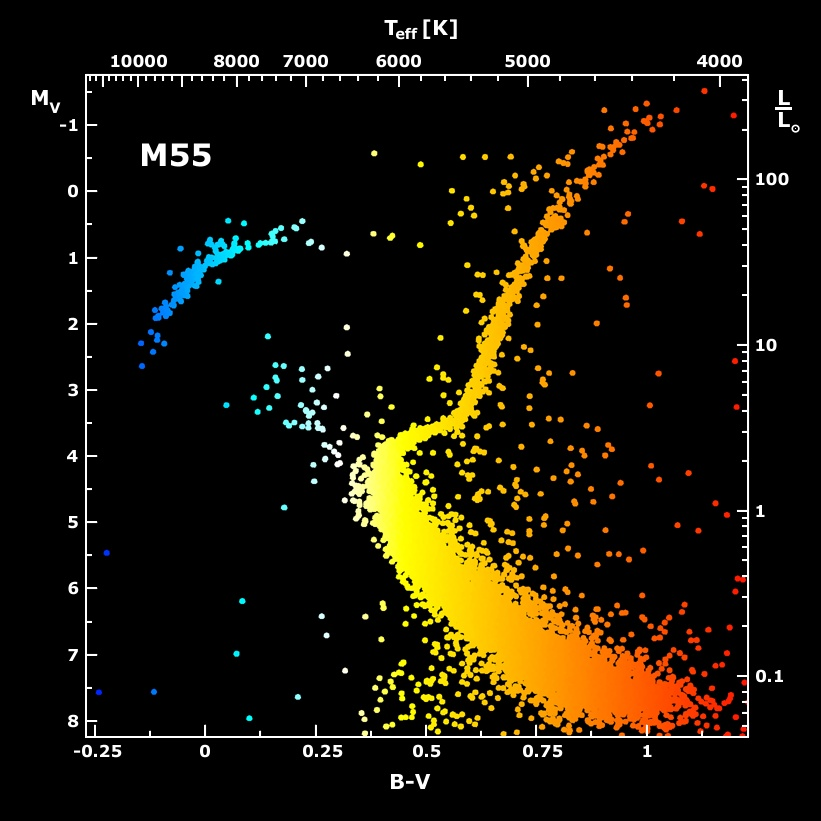
\includegraphics[width=\linewidth]{m55cmd_mochejska_big}
\caption[Color-magnitude diagram for the globular cluster M55]{\label{f.m55-cmd}Color-magnitude diagram for the globular cluster M55. \imgcred\ B.J. Mochejska, J. Kaluzny (CAMK), 1m Swope Telescope.}
\end{marginfigure}
Figure~\ref{f.m55-cmd} shows a color-magnitude diagram for the globular cluster M55. The figure plots the absolute $V$-band magnitude against the $(B-V)$ index---brighter and bluer stars at top left, dimmer and redder stars at lower right. The surface effective temperatures is indicated along the top axis, and the luminosity in solar units is indicated along the right axis.

Each dot on the plot represents a star, and the colors indicate how the star would appear. The main sequence forms a band running from the lower right to the center of the figure. At the time of the cluster's birth, the main-sequence would have continued on to the upper left of the plot.  Stellar mass increases as one moves upwards and leftwards along the main-sequance, and since more massive stars evolve faster, those bright, blue stars originally on the upper left of the main sequence have ended their hydrogen-burning tenure and moved on. From the location of the main-sequence turn-off, the age of the cluster is estimated\cite{VandenBerg2018Constraints-on-} to be $\val{12.9\pm0.8}{\Giga\yr}$. The red giant branch arcs from the center of the plot towards the upper right.  As stars turn away from the main sequence and their helium core mass grows, the stars move up the red giant branch becoming redder and more luminous.

\subsection{Helium burning: the horizontal branch}
There are no stable isotopes with mass number $A=5$ or $A=8$, which makes the fusion of \helium\ somewhat tricky. Although unstable, the isotope \beryllium[8] is relatively long-lived ($\val{10^{-16}}{\second}$) compared to a nuclear timescale\sidenote{Roughly the time for a pion to cross a nucleus, $\sim \val{10^{-22}}{\second}$.}. As a result,
when the core temperature reaches $\approx\val{10^{8}}{\K}$,\marginnote{The mass of a \beryllium[8] nucleus is $\val{91}{\kilo\eV}$ \emph{greater} than the mass of two \helium\ nuclei; at a temperature $\approx\val{10^{8}}{\K}$, the kinetic energy of the \helium\ nuclei is just enough to make up the difference.} the reaction
\[ \helium + \helium \longleftrightarrow\beryllium[8] \]
builds up a minute abundance of \beryllium[8]. This abundance is sufficient for the reaction
\[ \beryllium[8] + \helium \longleftrightarrow \carbon^{*} \]
to make a small abundance of \carbon\ in an excited state (denoted by the $^{*}$).  While most of the $\carbon^{*}$ decays back into $\beryllium[8]+\helium$, a small fraction decays instead to the ground state, $\carbon^{*}\to\carbon+\gamma$. The net result is $3\,\helium\to\carbon$, known as the \newterm{triple-alpha reaction}.

Once core \helium\ has ignited,\marginnote[-4\baselineskip]{The triple-alpha reaction is incredibly temperature-sensitive: $\partial\ln\epsilon_{3\alpha}/\partial\ln T \approx 40$ at $T = \val{10^{8}}{\K}$. This sensitivity, combined with the mildly degenerate conditions of the core, makes the ignition of \helium\ somewhat unstable for solar-mass stars.} the star settles onto a ``helium main sequence;'' observationally this is the \newterm{horizontal branch}, so called because these stars lie in a clump on a Hertzsprung-Russell diagram. The luminosity on the horizontal branch is about \valrng[--]{30}{100}{\Lsun}. The higher luminosity and the much lower energy release from the triple-alpha reaction make the horizontal branch lifetime much shorter than that of the main-sequence (e.g., the horizontal branch lifetime is $\sim \val{10^{8}}{\yr}$ for a solar-mass star). The horizontal branch is clearly visible as the blue arc in the upper-left quadrant of Fig.~\ref{f.m55-cmd}.

\begin{exercisebox}[Horizontal branch lifetime]
Use the result of exercise \ref{ex.energy-release} to find the heat released per kilogram from fusing 3 \helium\ nuclei into \carbon. Take the core mass to be $\val{0.45}{\Msun}$ (the minimum core mass needed for the ignition of helium), and find the lifetime for core helium burning for a horizontal branch luminosity of $\val{30}{\Lsun}$,.
\end{exercisebox}

\subsection{The asymptotic giant branch and emergence of a white dwarf}

As the mass of \carbon\ builds up in the core, the reaction $\carbon+\helium\to\oxygen$ begins to compete with the triple alpha reaction. As a result, the core becomes composed of a \carbon/\oxygen\ mixture.
With the depletion of \helium, the core---now composed of \carbon\ and \oxygen---again contracts, while the growing luminosity from the H- and He-burning shells again inflate the envelope to large radii. Observationally, this phase is the \newterm{asymptotic giant branch}: the stars move away from the horizontal branch and become redder and more luminous. This branch can be observed in Fig.~\ref{f.m55-cmd} arcing from the horizontal branch and asymptotically approaching the red giant branch at upper right. 

During the ascent of the asymptotic giant branch, the star's hydrogen-rich envelope is consumed at its base by the H- and He-burning shells and expelled at the surface by an increasingly strong wind. The expelled envelope resembles a nebula and is termed a \newterm{planetary nebula} (Fig.~\ref{f.NGC2392}). After the envelope has dispersed, the hot core---observed as a white dwarf---slowly cools. For a solar-mass star, the expected final mass of the core, and hence of the white dwarf, is $\approx\val{0.6}{\Msun}$.
\begin{marginfigure}
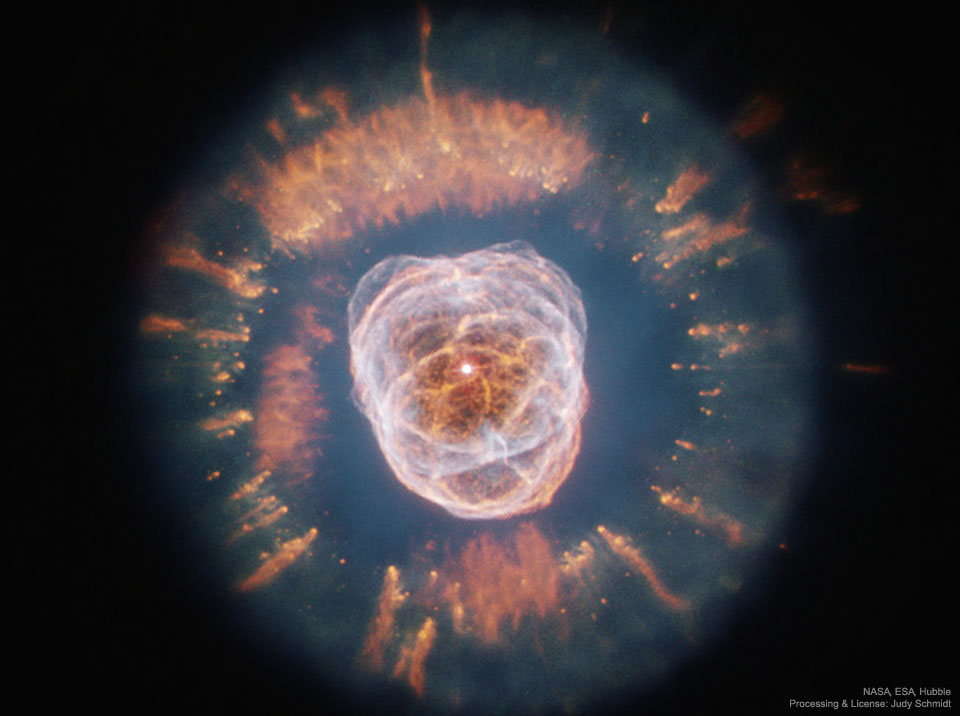
\includegraphics[width=\linewidth]{NGC2392_HubbleSchmidt_960}
\caption[The planetary nebula NGC 2392]{\label{f.NGC2392} The planetary nebula NGC~2392. \imgcred\ NASA, ESA, Hubble, Chandra; \emph{Processing \& \href{https://creativecommons.org/licenses/by/2.0/}{\ccby\ License}:} Judy Schmidt.}
\end{marginfigure}

\section{Massive stars}

For stars with main-sequence masses $\gtrsim \valrng[--]{8}{10}{\Msun}$, the fusion of \carbon\ commences while the core is non-degenerate and at a temperature $\approx\val{\sci{8}{8}}{\K}$.  At this temperature, electron-positron pairs form and annihilate ($e^{-}+e^{+}\longleftrightarrow\gamma\gamma$); occasionally instead of decaying into photons, the reaction
\[ e^{-}+e^{+} \longrightarrow \nu_{e} + \bar{\nu}_{e}\]
occurs instead and generates a neutrino-antineutrino pair. The mean free path for the neutrinos is larger than the radius of the star; as a result, the neutrinos stream out and take energy from the core. Because the neutrinos can easily leave the star, they end up carrying away the bulk of the heat from the core at these high core temperatures.

Within the core, \carbon\ is consumed by the reactions
\[ \carbon+\carbon\to\left\{\begin{array}{c}\sodium+\pt \\\neon+\helium\end{array}\right.. \]
The \pt\ and \helium\ capture onto other nuclei that are present.  At slightly higher temperatures, $\neon+\gamma \to \oxygen+\helium$ releases \helium\ nuclei that subsequently capture onto other \oxygen, \neon, and \magnesium. As the temperature increases, the next significant burning stage is
\[\oxygen+\oxygen\to\left\{\begin{array}{c}\phosphorus[31]+\pt \\ \silicon+\helium \end{array}\right. ;\]
as with $\carbon+\carbon$, the \pt\ and \helium\ combine with ambient nuclei with the end result being a distribution of isotopes about \silicon.

\begin{exercisebox}[Dynamical time of evolved stellar core]
At the onset of \oxygen\ burning in a \val{25}{\Msun} star, the central density (Table~\ref{t.burning-timescales}) is $\val{\sci{3.6}{9}}{\kilo\gram\,\meter^{-3}}$.  What is the dynamical time of the core?
\end{exercisebox}

The strong Coulomb barrier inhibits the fusion of nuclei beyond \oxygen; instead, photodissociation reactions such as $\silicon+\gamma \to \magnesium+\helium$ liberate \nt, \pt, and \helium.  These light nuclei then capture onto heavier nuclei, and the composition gradually becomes composed of isotopes about \iron.  This is \newterm{nuclear statistical equilibrium}: the composition is in the lowest energy state (most bound) for the ambient density and temperature. As a result, there is no further release of nuclear energy possible. The (mostly \iron) core contracts and becomes degenerate; its mass gradually increases from the burning of surrounding material.

The amount of energy available from the reactions with heavy nuclei is low; as a consequence, the time required for the core to deplete the available fuel grows shorter and shorter, with the final stages occurring in a day (column labeled $\tau$ in Table~\ref{t.burning-timescales}). After the ignition of carbon, the core evolves too quickly for the envelope to keep up. Thus the external appearance of the star provides no window into the final days of burning.

\begin{table}[htp]
\forcerectofloat\small
\caption[Nuclear burning timescales for massive stars]{\label{t.burning-timescales}Nuclear burning timescales for massive stars. Values taken from \citet{Woosley2002The-evolution-a}; neutrino luminosities are taken from \citet{Weaver1978Presupernova-ev} and do not exactly correspond to the same stellar models for the other parameters.}
\begin{tabular}{rrrrrr}
\multicolumn{5}{c}{hydrogen}\\
\hline
$M_{\mathrm{ZAMS}}$ & $T_{c}$ & $\rho_{c}$ & $L$ & $L_{\nu}$ & $\tau$\\
\Msun & $\val{10^{7}}{\K}$ & $\val{10^{3}}\kilo\gram\,\meter^{-3}$ & $\val{10^{3}}{\Lsun}$ & \Lsun & Myr\\
\hline
15 & 3.53 & 5.81 & 28 & --- &11.1\\
25 & 3.81 & 3.81 & 110 & --- & 6.7\\
\hline\hline
\multicolumn{5}{c}{helium}\\
\hline
$M_{\mathrm{ZAMS}}$ & $T_{c}$ & $\rho_{c}$ & $L$ & $L_{\nu}$ & $\tau$ \\
\Msun & $\val{10^{8}}{\K}$ & $\val{10^{6}}{\kilo\gram\,\meter^{-3}}$ & $\val{10^{3}}{\Lsun}$ & $\Lsun$ & Myr\\
\hline
15 & 1.78 & 1.39 & 41 & 1 &1.97\\
25 & 1.96 & 0.76 & 182 & 20 & 0.84\\
\hline\hline
\multicolumn{5}{c}{carbon}\\
\hline
$M_{\mathrm{ZAMS}}$ & $T_{c}$ & $\rho_{c}$ & $L$ & $L_{\nu}$ & $\tau$ \\
\Msun & $\val{10^{8}}{\K}$ & $\val{10^{9}}{\kilo\gram\,\meter^{-3}}$ & $\val{10^{3}}{\Lsun}$ & $\val{10^{3}}{\Lsun}$ & kyr \\
\hline
15 & 8.34 & 2.39 & 83 & 90 & 2.03\\
25 & 8.41 & 1.29 & 245 & 2600 & 0.52\\
\hline\hline
\multicolumn{5}{c}{oxygen}\\
\hline
$M_{\mathrm{ZAMS}}$ & $T_{c}$ & $\rho_{c}$ & $L$ & $L_{\nu}$ & $\tau$ \\
\Msun & $\val{10^{9}}{\K}$ & $\val{10^{9}}{\kilo\gram\,\meter^{-3}}$ & $\val{10^{3}}{\Lsun}$ & $\val{10^{6}}{\Lsun}$ & yr\\
\hline
15 & 1.94 & 6.66 & 87 & 2 & 2.58\\
25 & 2.09 & 3.60 & 246 & 6000 & 0.40\\
\hline\hline
\multicolumn{5}{c}{silicon}\\
\hline
$M_{\mathrm{ZAMS}}$ & $T_{c}$ & $\rho_{c}$ & $L$ & $L_{\nu}$ & $\tau$ \\
\Msun & $\val{10^{9}}{\K}$ & $\val{10^{10}}{\kilo\gram\,\meter^{-3}}$ & $\val{10^{3}}{\Lsun}$ & $\val{10^{6}}{\Lsun}$ & d\\
\hline
15 & 3.34 & 4.26 & 87 & $10^{5}$ & 18.3\\
25 & 3.65 & 3.01 & 246 & $10^{6}$ & 0.7\\
\end{tabular}
\end{table}

\begin{marginfigure}
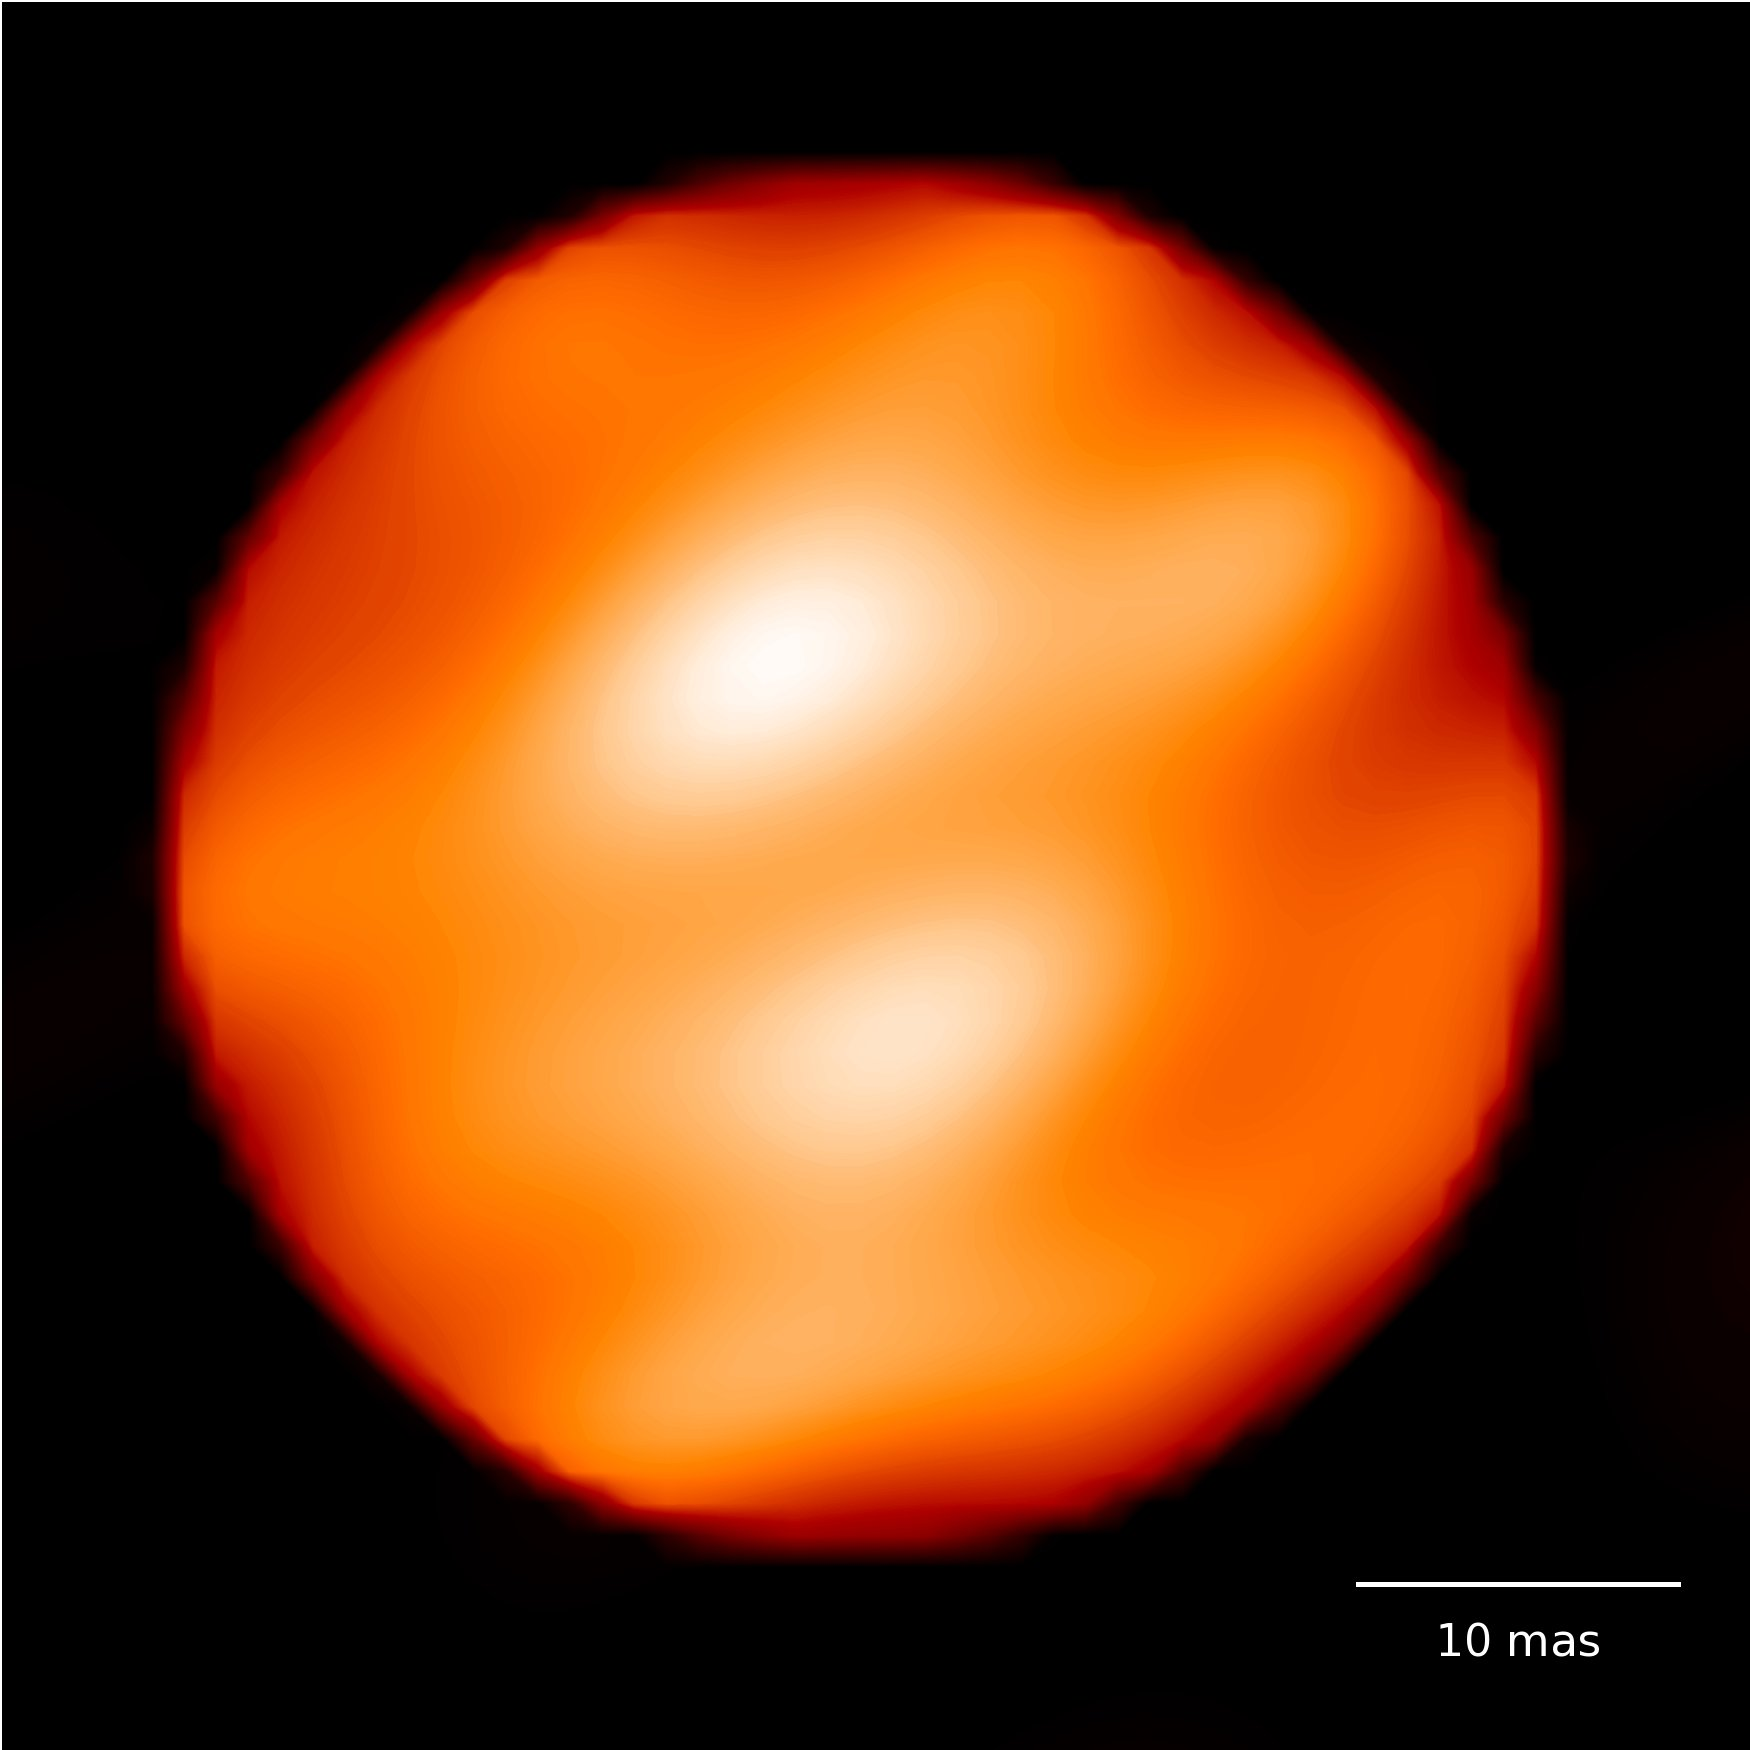
\includegraphics[width=\linewidth]{Betel_haubois}
\caption[Betelgeuse]{\label{f.betelgeuse} A reconstructed image of Betelgeuse made using interferometry. \imgcred\ Xavier Haubois et al. (Observatoire de Paris)}
\end{marginfigure}
The best-known example of an evolved massive star is Betelgeuse, which is large enough and close enough to be resolved (Fig.~\ref{f.betelgeuse} shows a reconstructed image made with interferometry). Betelgeuse probably started as a blue main-sequence star of approximately $\val{20}{\Msun}$ and is now burning helium in its core now. The extended envelope, $\approx\val{5}{\AU}$ in radius, has large convective cells (bright spots in image) and pulsates violently. As can be inferred from Table~\ref{t.burning-timescales}, in less than $\val{1}{\Mega\yr}$ Betelgeuse's core will reach nuclear statistical equilibrium; no more nuclear energy will be available and Betelgeuse will transform into either a neutron star or black hole, as we describe next.

\subsection{Core collapse}
When the core of a massive star reaches nuclear statistical equilibrium, there are no further sources of energy available. Fusion reactions in the shells surrounding the core add mass to it, causing it to contract. The increasing density raises the electron Fermi energy. When the Fermi energy approaches the rest mass of the electrons---$m_{e}c^{2} = \val{0.511}{\MeV}$---the electrons move relativistically. This dramatically alters the equation of state.

A particle's energy, including rest mass, is
\[
	E = \sqrt{p^{2}c^{2} + m^{2}c^{4}} = mc^{2}\left[1 + \left(\frac{p}{mc}\right)^{2}\right]^{1/2};
\]
when $p\ll mc$, we can expand this as $E\approx m c^{2} + p^{2}/2m$---that is, as the sum of the rest mass and the Newtonian kinetic energy. In the opposite limit, when $p \gg mc$, $E \approx pc$. Let's see how this relativistic limit affects the degenerate equation of state. Recall that we fill energy states, starting with the lowest open levels until we have added all $N$ electrons (eq.~[\ref{e.number-degenerate}]):
\[
	N = \frac{2}{h^{3}}\int_{V}\dif^{3}x\int_{0}^{\EF}\dif^{3}p.
\]
Change variables, $\dif^{3}p = 4\pi p^{2}\,\dif p = 4\pi c^{-3}\varepsilon^{2}\,\dif\varepsilon$, where $\varepsilon = pc$ is the energy of a single, relativistic electron:
\[
	N = \frac{8\pi}{h^{3}c^{3}}V \int_{0}^{\EF} \varepsilon^{2}\,\dif\varepsilon
	= \frac{8\pi}{3h^{3}c^{3}} V  \EF^{3}.
\]
This gives the Fermi energy,
\[
	\EF = hc\left(\frac{3}{8\pi}\frac{N}{V}\right)^{1/3}.
\]
To get the total energy, multiply each electron by its energy $\varepsilon$ and integrate over phase space:
\[
	E = \frac{8\pi}{h^{3}c^{3}}V\int_{0}^{\EF}\varepsilon^{3}\,\dif\varepsilon = 
		\frac{1}{4}\frac{8\pi}{h^{3}c^{3}}V\EF^{4} = \frac{3}{4}N\EF.
\]
For a relativistic gas, the pressure is $P = (1/3)(E/V)$ (cf.\ Box~\ref{sb.radiation-pressure}), so that
\begin{equation}
\label{e.pressure-relativistic}
	P = \frac{1}{4}n\EF = \frac{1}{4}\left(\frac{3}{8\pi}\right)^{1/3}hc n^{4/3},
\end{equation}
with $n = \rho/\mu_{e}m_{u}$. Instead of $P\propto\rho^{5/3}$, as for a non-relativistic gas, $P\propto\rho^{4/3}$.

\subsection{The Chandrasekhar mass}

In exercise~\ref{ex.degenerate-mass-radius}, we constructed a mass-radius relation for white dwarfs by combining the virial relations,
\begin{eqnarray*}
   P    &\propto& \frac{GM^{2}}{R^{4}}\\
   \rho &\propto& \frac{M}{R^{3}}
\end{eqnarray*}
and the equation of state for a non-relativistic, degenerate, ideal gas.  We found that $R\propto M^{-1/3}$.  If we try that with our relativistic equation of state, eq.~(\ref{e.pressure-relativistic}), we get
\[
	\frac{GM^{2}}{R^{4}} \propto P = \frac{1}{4}\left(\frac{3}{8\pi}\right)^{1/3}hc\; \left(\frac{\rho}{\mb\mu_{e}}\right)^{4/3} \propto \frac{hc}{\mb^{4/3}}\frac{M^{4/3}}{R^{4}}.
\]
The radius $R$ cancels, and what we have is a relation $M\propto (hc/G)^{3/2}/\mb^{2}$.  This is rather odd: a gas with a relativistic equation of state in hydrostatic balance has a characteristic mass defined in terms of fundamental constants.

Let's investigate this further. Suppose we have a box with adjustable sides, which we pack with $N$ degenerate electrons. We add some nuclei for mass, so that the total mass in the box is $\mu_{e}\mb N$. The volume of the box $V \sim R^{3}$, and since the electrons are degenerate, the volume per electron is roughly $\lambda^{3}$, where $\lambda \sim h/p$ is the wavelength of the electrons.  As a result, $N = (R/\lambda)^{3}$; further, the momentum of an electron is
\[	p \sim \frac{h}{\lambda} \sim h\frac{N^{1/3}}{R}. \]
If our electrons were non-relativistic, the total, kinetic plus gravitational, energy of our box would be
\[
	E_{\mathrm{total}} = N\frac{p^{2}}{2m_{e}} - \frac{GM^{2}}{R} \sim N^{5/3}\frac{h^{2}}{R^{2}m_{e}} - GN^{2}\mu_{e}^{2}\mb^{2} \frac{1}{R}.
\]
For a given $N$, we can adjust $R$ to make $E_{\mathrm{total}}<0$, and indeed, if we satisfy the virial theorem, we will recover the $R\propto M^{-1/3}$ scaling.

If, however, the electrons are relativistic then the total energy is
\begin{eqnarray*}
	E_{\mathrm{total}} = Npc - \frac{GM^{2}}{R} 
		&=& \frac{1}{R}\left[hc N^{4/3} - G N^{2}(\mu_{e}\mb)^{2}\right]\\
		&=& G(\mu_{e}\mb)^{2}\frac{N^{4/3}}{R}
		{\color{red}\left[ \frac{hc}{G(\mu_{e}\mb)^{2}} - N^{2/3}\right]}.
\end{eqnarray*}
Look at the term in $\color{red}\left[\cdot\right]$.
If $N < [hc/G/(\mu_{e}\mb)^{2}]^{3/2}$, then $E_{\mathrm{total}} > 0$; by making $R$ larger, however, we can lower the energy until the electrons are no longer relativistic, and then we can again recover the virial scaling.  If $N > [hc/G(\mu_{e}\mb)^{2}]^{3/2}$ then $E_{\mathrm{total}} < 0$; by making $R$ smaller, however, we can keep reducing $E_{\mathrm{total}}$ indefinitely. 
\begin{quote}\itshape
There is no bound state with finite $R$ for $M>(hc/G)^{3/2}(\mu_{e}\mb)^{-2}$.
\end{quote}

\begin{sidebar}[Instability for a relativistic equation of state]
There is another way of looking at the onset of instability which is instructive (this treatment follows that in \citet{Cox1980Theory-of-Stell}). In exercise \ref{ex.stellar-oscillation-period} you found that during a contraction or expansion, the equation of motion for a thin layer at the star's surface was
\[
	\ddot{\delta R} = \frac{GM}{R^{2}}\left[4-3\gamma\right]\frac{\delta R}{R}.
\]
Here $M$ and $R$ are the total stellar mass and radius, and the adiabatic pressure-density relation is $P\propto \rho^{\gamma}$.

For a non-relativistic gas with $\gamma = 5/3$, we have $\ddot{\delta R} \propto -\delta R$: the star oscillates with a period that is comparable to the dynamical timescale of the star. If, however, $\gamma < 4/3$ the equation of motion is $\ddot{\delta R} \propto \delta R$, which has an exponential solution: squeeze the star slightly, and it will implode!

Let's work out a more physical explanation for what is happening. Suppose we have a star in virial equilibrium, with the central pressure and density
\begin{eqnarray*}
P &\propto& \frac{GM^{2}}{R^{4}} \\
\rho &\propto& \frac{M}{R^{3}}.
\end{eqnarray*}
Now if the star contracts by a small amount, say $\delta R/R = -1\%$, then the density increases by an amount $\delta\rho/\rho = -3\delta R/R = 3\%$. How does the pressure respond? If the star contracts slowly, on a Kelvin-Helmholtz timescale, then there is time for heat to radiate away, so that the internal pressure can increase by the amount needed to maintain virial equilibrium: in this case $\delta P/P = -4\delta R/R = 4\%$. Under an \emph{adiabatic} contraction, however, there is not enough time for the star to radiate away excess heat; as a consequence, the pressure and density are linked, so that $\delta P/P = \gamma\delta \rho/\rho = -3\gamma\delta R/R$.

If the adiabatic index is $\gamma = 4/3$, then during an adiabatic compression of $\delta R/R = -1\%$, the density increases by $3|\delta R/R| = 3\%$ and the pressure increases by $3\gamma|\delta R/R| = 4\%$, which is precisely the increase needed to maintain mechanical equilibrium. As a result, the star remains in hydrostatic balance at its new, smaller radius. This is why there was no mass-radius relation for $\gamma = 4/3$; it takes no energy to contract (or expand) the star.

For $\gamma > 4/3$, the central pressure increases during contraction by $3\gamma|\delta R/R| > 4|\delta R/R|$. As a result, the pressure becomes greater than the amount needed for hydrostatic balance. This excess pressure pushes the star outward and acts as a restoring source. During an expansion, the pressure falls below the amount needed for hydrostatic equilibrium, so gravity halts the expansion and forces the star to contract. Hence, for $\gamma > 4/3$, the star responds to a radial perturbation by oscillating with a period comparable to the dynamical timescale (cf.\ exercise \ref{ex.stellar-oscillation-period}).

In contrast, if $\gamma < 4/3$ the increase in pressure during contraction is $3\gamma|\delta R/R| < 4|\delta R/R|$. The gas pressure does not increase enough to maintain hydrostatic equilibrium, and so the star's contraction accelerates. A small perturbation inwards leads to implosion.
\end{sidebar}

Thus, there is a limit to the total mass that can be supported in hydrostatic equilibrium by degenerate electrons. 
An exact calculation for the maximum mass of a cold, degenerate star yields
\begin{equation}\label{e.Chandrasekhar}
	M_{\mathrm{Ch}} = 1.456 \left(\frac{2}{\mu_{e}}\right)^{2}\Msun.
\end{equation}
When the mass reaches this limiting value, known as the \newterm{Chandrasekhar mass}\sidenote{Derived by S. Chandrasekhar at age 20(!) while traveling from India to England in 1930}, the electrons become relativistic and $\partial P/\partial \rho \to 4/3$; the star becomes unstable and collapses.

When the core of a massive star begins its collapse, the electron Fermi is $\sim\MeV$, which is sufficient to induce electron captures on iron-group nuclei. These captures increase $\mu_{e}$ and reduce $M_{\mathrm{Ch}}$. As the core begins the final plunge, the rapidly rising temperature induces the photodissociation of iron-group nuclei into neutrons, protons, and helium nuclei. This process is endothermic, which further robs the core of pressure support and accelerates the collapse. The effective $\gamma = \partial P/\partial\rho < 4/3$ on account of the photodissociation and electron captures, and the core implodes.

As the core density approaches $\val{0.16}{\fermi^{-3}}$,\marginnote{the density of an atomic nucleus} the nucleons begin to repel one another on account of the strong nuclear force. This abruptly halts the collapse and launches a shockwave outwards. The core now consists mostly of neutrons and is termed a \newterm{neutron star}.

\begin{exercisebox}[Gravitational binding energy of a neutron star]
What is the mass density if the number density of nucleons is $\val{0.16}{\fermi^{-3}}$? What is the gravitational binding energy for an object with a mass \val{1.4}{\Msun} at this density?
\end{exercisebox}

The outward traveling shockwave soon stalls as the outer layers of the star fall inward. The energy needed to blow the envelope off is about 1\% of the gravitational binding energy of the core, so there is plenty of energy available to disperse the envelope if this energy can be tapped. Most of the gravitational binding energy released by the imploding core is carried outwards by neutrinos. This has been confirmed observationally\cite{Arnett1989Supernova-1987A}. In February 1987 the star Sk~-69\,202, a B3 supergiant in the Large Magellanic Cloud, became supernova 1987A. Just before the optical brightening, a burst of neutrinos were detected in 
the Kamiokande II (Japan) and IMB (Ohio) water Cherenkov detectors.

During the collapse, the neutrino mean free path becomes smaller than the core radius for two reasons: the weak interaction cross-section increases as the nucleons reach temperatures $\gtrsim\val{10^{10}}{\K}$, and the mean free path $\ell = (n\sigma)^{-1}$ decreases as the density rises.
As a result, the neutrinos become trapped and must diffuse out of the collapsing core. As the neutrinos diffuse out, they transfer a small fraction of their energy to the material, which heats it. This heating tends to push the shock outward, and a competition arises between the ram pressure of infalling matter and the heating from the neutrinos. If the neutrinos can transfer enough energy to the envelope, then the envelope will be blown off in a supernova. If not, then matter will continue to accumulate onto the neutron star. The maximum mass of a neutron star is uncertain\sidenote{By timing pulsars (next section) in a binary system, the orbital parameters and hence the mass of the neutron star can be deduced; the largest measured mass is $\val{2.14_{-0.09}^{+0.10}}{\Msun}$ \citep{Cromartie2020Relativistic-Sh}.}, but on physical grounds is likely $< \val{3}{\Msun}$. If the shock is not re-energized, then conceivably the entire star could implode into a black hole---the star would disappear without a corresponding luminous supernovae. There is evidence that this has happened\cite{Adams2017The-search-for-}.

\section{Stellar resurrection}
\label{s.stellar-resurrection}

In the previous section, we learned that stars with $M\lesssim\valrng[--]{8}{10}{\Msun}$ eventually become white dwarfs composed of carbon and oxygen and supported by electron degeneracy pressure; and that more massive stars have cores that collapse, either to form neutron stars supported by the strong nuclear interaction or to collapse fully into black holes.

Both the white dwarfs and neutron stars that emerge from the ashes of isolated stars slowly cool and dim. The cooling of white dwarfs can be modeled accurately enough that observations of white dwarfs in clusters can be used to infer the ages of and distances to their host clusters. No such capability is possible with isolated neutron stars: most are too dim to be observed, and there are vast uncertainties about the composition of the deep interior, where the density is several times higher than that of an atomic nucleus. Rather, efforts have been on using observations of the handful of isolated neutron stars with measured surface temperatures to constrain models of nuclear matter.

\begin{marginfigure}[-10\baselineskip]
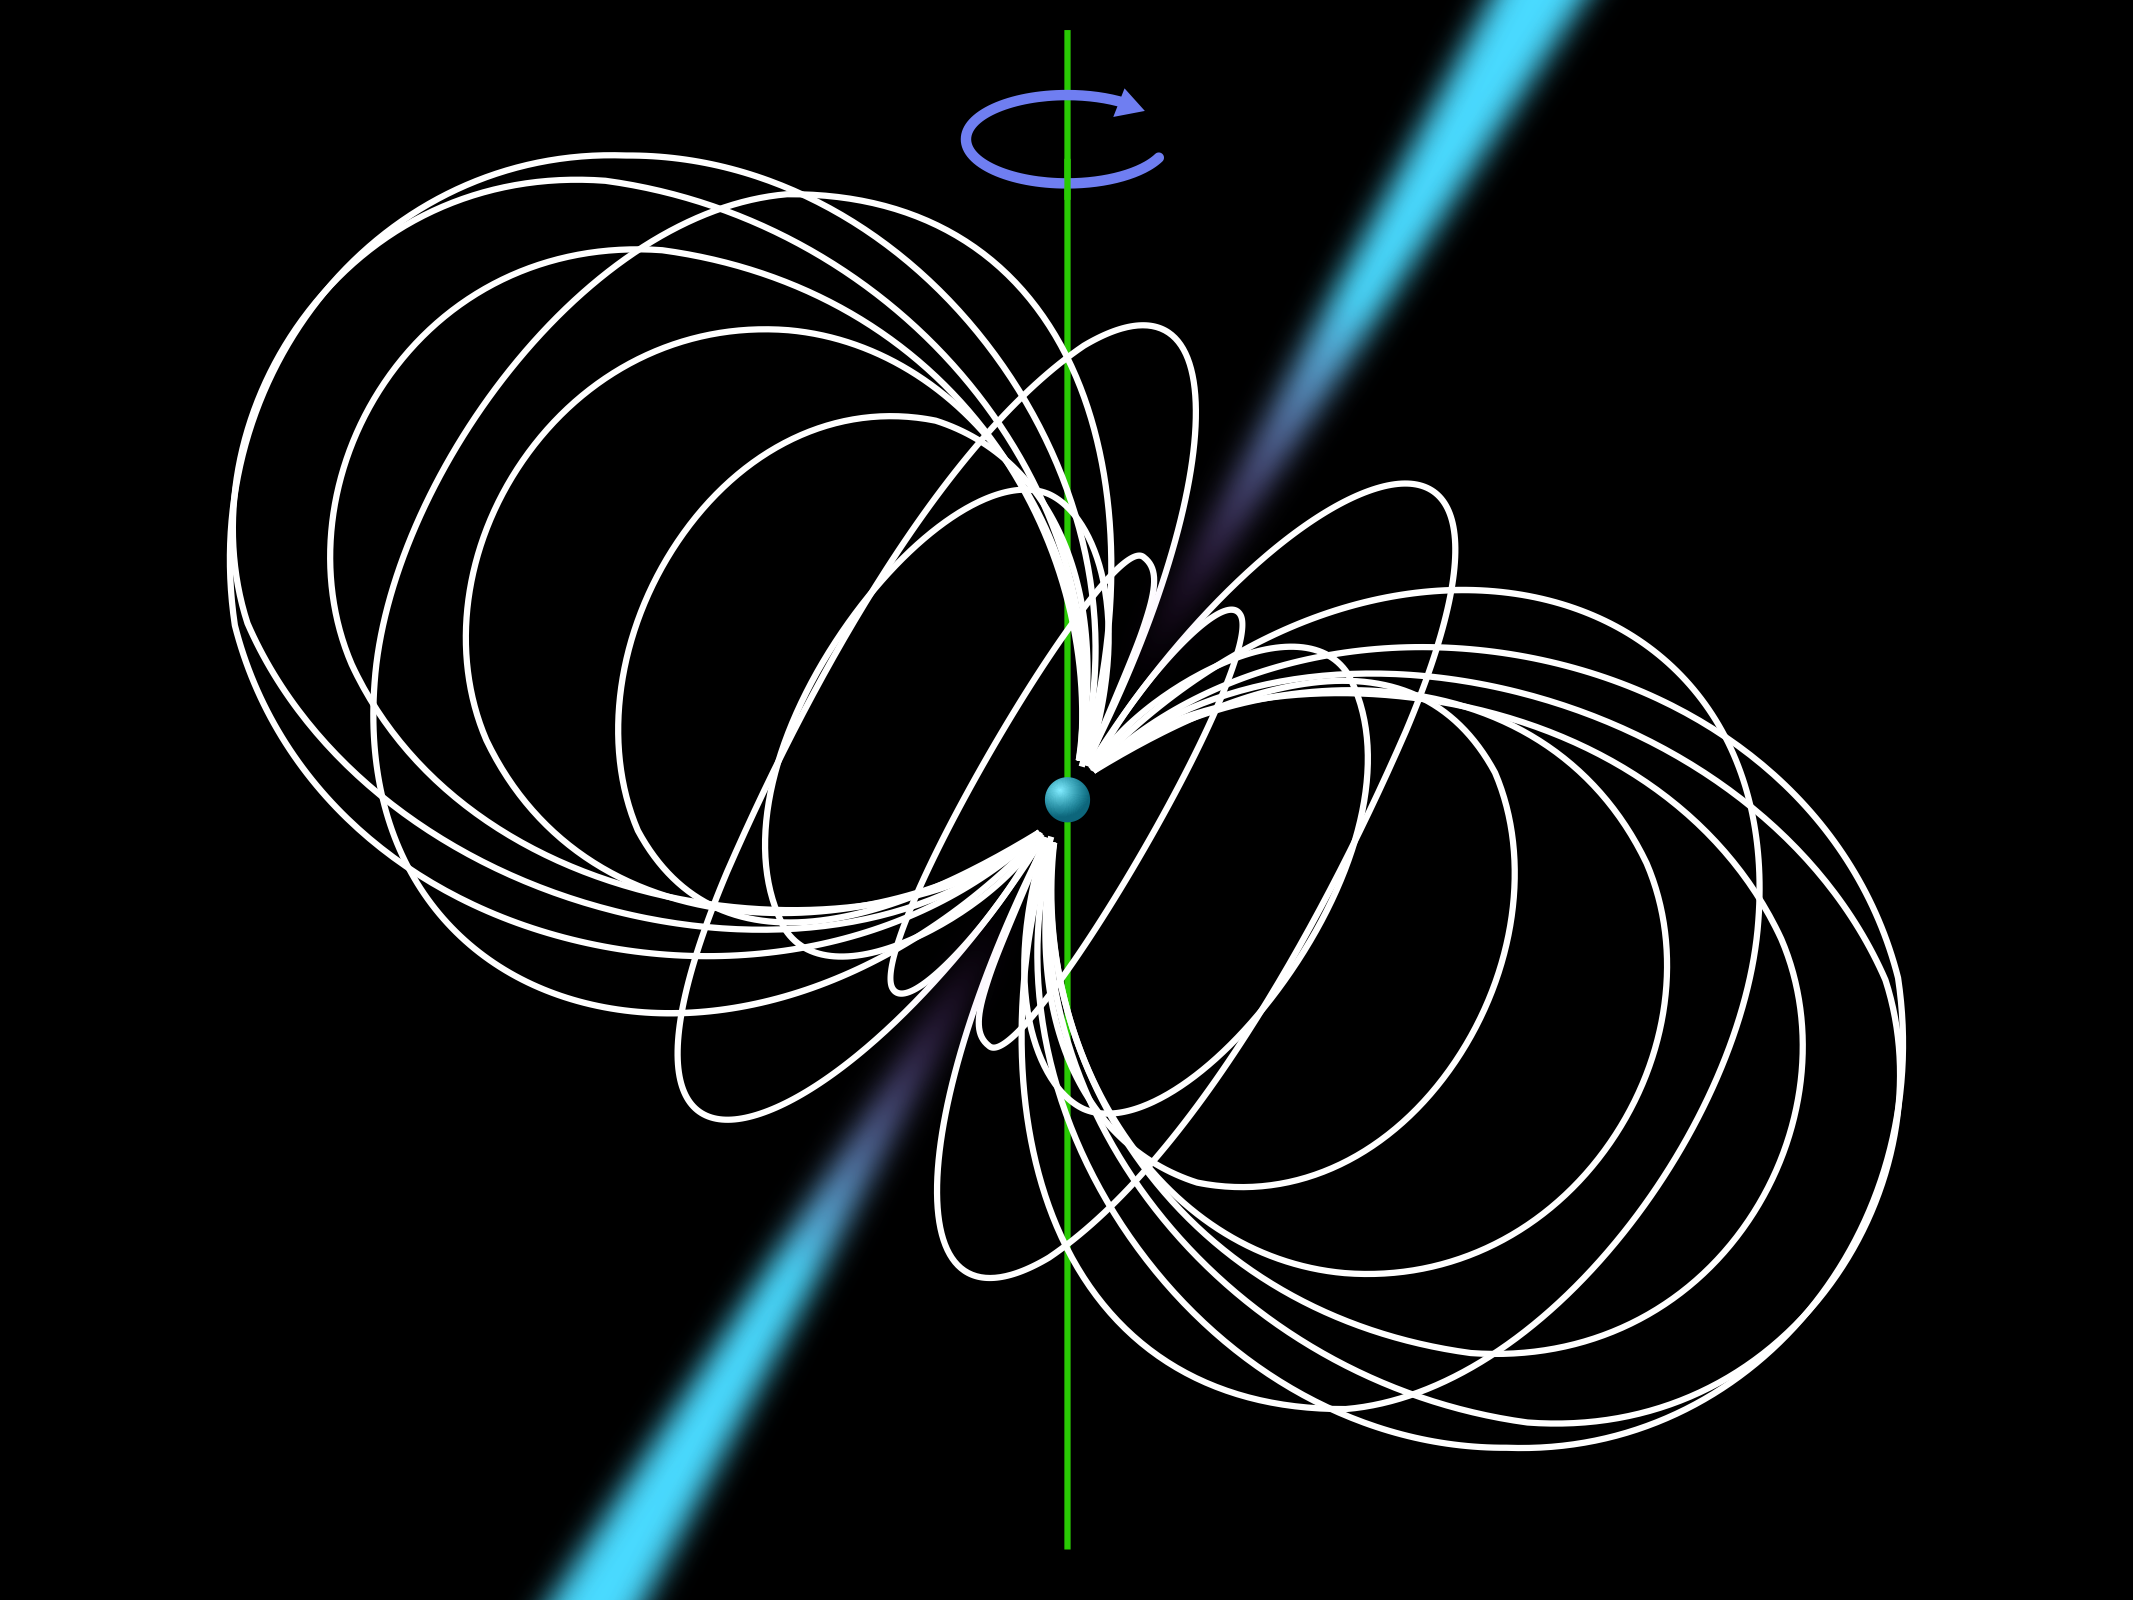
\includegraphics[width=\linewidth]{Pulsar_schematic}
\caption[Schematic of a pulsar]{\label{f.pulsar-schematic}
Schematic of a pulsar. The white lines indicate the dipole magnetic field, the green line is the rotation axis, and the light blue beams are the radiation. \imgcred\ Made by Mysid in Inkscape, based on \texttt{Pulsar schematic.jpg} by Roy Smits. \href{https://creativecommons.org/licenses/by-sa/3.0/}{\ccbysa}.}
\end{marginfigure}
Many observed neutron stars are endowed with strong magnetic fields, with a surface dipole field strength $\gtrsim\val{10^{8}}{\unitstyle{T}}$. If the neutron star spins rapidly enough and the dipole is misaligned with the spin axis, a tremendous voltage is generated at the surface that accelerates charges above the polar caps. These accelerated charges emit photons that fan outward from the poles, as illustrated in Fig.~\ref{f.pulsar-schematic}. As the neutron star spins, the beams of radiation are swept around; a distant observer therefore observes light pulsing at the rotation frequency of the star. These systems, known as \newterm{pulsars}, were discovered by Jocelyn Bell\sidenote{Jocelyn Bell was a 24 year old graduate student at Cambridge at the time}
and Anthony Hewish in 1967\cite{Hewish1968Observation-of-}.
\marginnote{The radio emission from several pulsars, including the Crab, was independently detected by Airman C. Schisler at the Ballistic Missile Early Warning Site, Clear Air Force Station, Alaska.}

\begin{exercisebox}[Limiting spin frequency]
The Crab pulsar spins at \val{33}{\Hz}. For a star of \val{1}{\Msun}, find the maximum radius such that material at the equator remains bound to the star when spinning at that rate. Based on these results, argue that the Crab pulsar cannot be a white dwarf.
\end{exercisebox}

\newthought{Many stars are in binary systems.} If the binary happens to survive the evolution off the main sequence, it can often happen that the orbit is close enough for matter to be tidally stripped from the companion and \newterm{accreted} onto the compact star (i.e., white dwarf, neutron star, or black hole). As matter falls into the gravitational potential, it liberates a considerable amount of energy. This makes the system bright.

\begin{exercisebox}[Accretion onto a neutron star]
Let's estimate the luminosity and surface temperature of an accreting neutron star.
Assume a mass of \val{1.4}{\Msun} and a radius of \val{10}{\kilo\meter}. 
\begin{enumerate}
\item Compute the gravitational energy (in MeV) released when a proton falls onto the surface (use a Newtonian approximation for the gravitational potential). How does this compare to the energy released (per proton) from the fusion of hydrogen into helium?
\item Now suppose the neutron star is accreting \val{10^{14}}{\kilo\gram\usk\second^{-1}}, which is a typical rate for many observed systems. What would be the luminosity generated by this accretion? 
\item Suppose the luminosity were emitted thermally from the surface of the neutron star. What would be the surface effective temperature? In what band (e.g., visible, IR, UV, X-ray) would you want to observe this system?
\end{enumerate}
\end{exercisebox}

When sufficient material\sidenote{The accreted matter is usually mostly hydrogen, but if the companion star is evolved it could be enriched in helium or even, if the companion star is itself a white dwarf, carbon and oxygen.} has accumulated on the surface of a white dwarf or neutron star, thermonuclear reactions can ignite in the accreted layer. This ignition is typically thermally unstable and leads to an explosion. On a white dwarf, this explosion presents as a \newterm{nova}\sidenote{from the Latin \emph{novus} meaning ``new''} as the white dwarf abruptly brightens and then dims over several weeks to months. The mass of the burning layer is typically \valrng{10^{-5}}{10^{-4}}{\Msun}; at typical accretion rates $\lesssim\val{10^{-9}}{\Msun\usk\yr^{-1}}$ the time between the explosions is thousands of years or longer. The amount of mass necessary for ignition decreases strongly with the mass of the white dwarf, however, so that the time between explosions can be years to decades. In these systems the novae are observed to reoccur and they are called---appropriately enough---\newterm{recurrent novae}.
On a neutron star, the explosion is observed as an \newterm{X-ray burst} that lasts \valrng[--]{10}{100}{\second}. The strong gravity makes the amount of material needed for ignition much less than on a white dwarf: roughly \val{10^{-12}}{\Msun}. As a consequence, the time between bursts can be as short as hours to days. 

\newthought{Some neutron stars and black holes are in tight (short orbital period) binaries} with another neutron star or black hole. In this case, the system has an oscillating mass quadrupole; further, just as an oscillating electrical dipole radiates electromagnetic waves (light), the orbiting stars will radiate \newterm{gravitational radiation}. The gravitational radiation carries energy away from the binary and forces the orbit to shrink. As the orbit shrinks, the emission of gravitational radiation intensifies, and the rate of orbital shrinkage increases. Monitoring of the orbital period of the binary pulsar PSR~1913+16\cite{Hulse1975Discovery-of-a-} found that the orbital period, and hence the semi-major axis, were indeed decreasing at a rate consistent with predictions from General Relativity\cite{Taylor1982A-new-test-of-g}.

Direct detection of gravitational radiation was finally achieved in 2015 by the LIGO\sidenote{Laser Interferometer Gravitational-Wave Observatory} and Virgo gravitational wave observatories. The event GW150914 was the merger of two black holes with masses $\val{36_{-4}^{+5}}{\Msun}$ and $\val{29_{-4}^{+4}}{\Msun}$\cite{Abbott2016Observation-of-}. Two years later LIGO and Virgo observed the merger of two neutron stars, GW170817\cite{Abbott2017GW170817:-Obser}. The event was also detected in the $\gamma$-ray, X-ray, optical and infrared bands\cite{Abbott2017Multi-messenger}. The fading afterglow of the merger is consistent with the ejecta containing large amounts of high-opacity lanthanides. This suggests that the copious amounts of heavy elements were formed in the merger, and that perhaps such mergers are the origin of elements such as gold, platinum, and lead.  Your jewelry may be a souvenir of the violent merger of two neutron stars long ago.
